\documentclass[11pt, oneside]{article} 
\usepackage{geometry}
\geometry{letterpaper} 
\usepackage{graphicx}
	
\usepackage{amssymb}
\usepackage{amsmath}
\usepackage{parskip}
\usepackage{color}
\usepackage{hyperref}

\graphicspath{{/Users/telliott/Github/calculus_book/png/}}
% \begin{center} 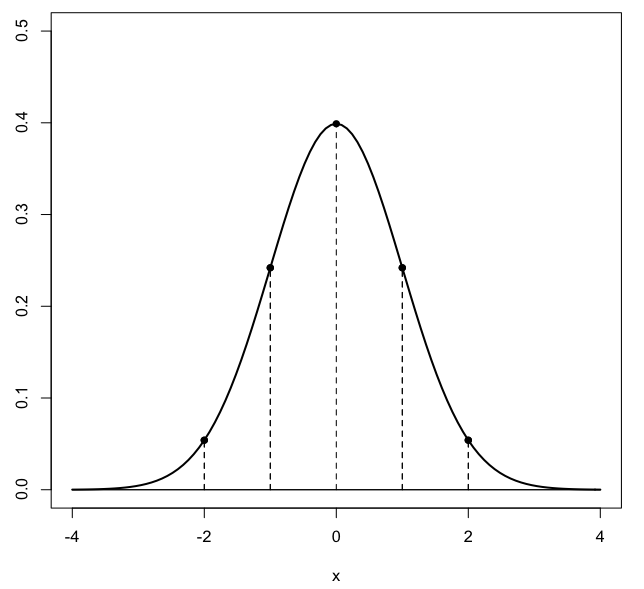
\includegraphics [scale=0.4] {gauss3.png} \end{center}

\title{Arcs of a circle}
\date{}

\begin{document}
\maketitle
\Large
From a previous chapter, Euclid's third postulate was:

$\circ$   Given any straight line segment, a circle can be drawn having the segment as radius and one endpoint as center.  The tool to do this is called a compass:

\url{https://en.wikipedia.org/wiki/Compass_(drawing_tool)}

If the radius is extended so that it cuts the circle at two points, it is called a diameter.  We saw previously that one can construct a line perpendicular to any given line.  If that line is constructed perpendicular to the diameter at the point where it meets the circle, the new line is called a tangent line.  By definition, the tangent line touches the circle at a single point.

\subsection*{arcs of a circle}

\begin{center} 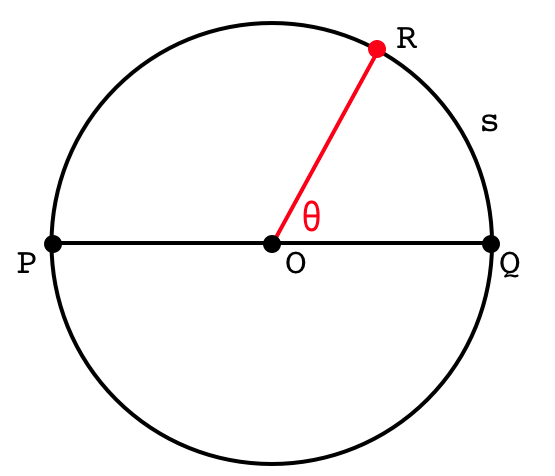
\includegraphics [scale=0.30] {arcs1.png} \end{center}
In calculus and analytical geometry angles are defined in terms of radians of arc. For a unit circle with radius = $1$, the total circumference is $2\pi$, so the arc swept out by the angle $\theta$ is in the same ratio to $2 \pi$ as the ratio of the angle's measure in degrees to $360^\circ$.

It seems natural then to adopt the arc length as a measure of the angle, where $360^\circ$ is equal to $2 \pi$ \emph{radians}, and an angle of $90^\circ$, for example, a right angle, is equal to $\pi/2$ radians.

\begin{center} 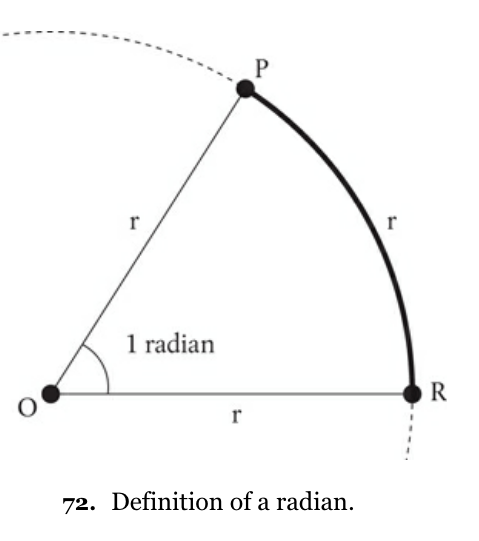
\includegraphics [scale=0.30] {radian.png} \end{center}

We say that the angle $\theta$ is equal to the arc it sweeps out on the circumference, in radians.
\[ s = \theta \]

To convert some more measures of angles in degrees to radians:
\[ 180^\circ = \pi, \ 90^\circ = \frac{\pi}{2} \]
\[ 60^\circ = \frac{\pi}{3}, \ 45^\circ = \frac{\pi}{4}, \ 30^\circ = \frac{\pi}{6} \]

\subsection*{Thales' theorem}

In this chapter, we introduce a few more theorems concerning circles, starting with the last of Thales' theorems:

$\circ$  Any angle inscribed in a semicircle is a right angle.

Now, think of three points on the circumference of the circle as forming a triangle. If two points are on a diameter of the circle, the angle formed at any arbitrary but distinct third point is always a right angle.

To prove: $\angle PRQ$ is a right angle.
\begin{center}
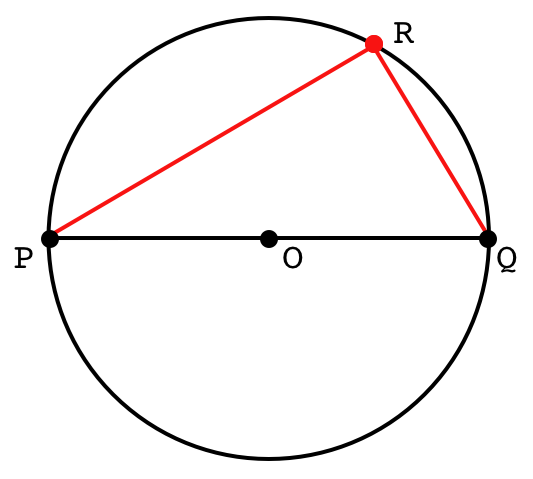
\includegraphics [scale=0.25] {arcs2.png} 
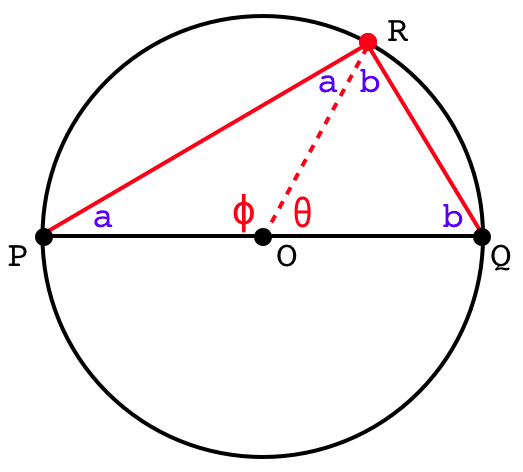
\includegraphics [scale=0.25] {arcs3.png}
\end{center}
Solution:
Draw the radius OR. Notice that $\triangle OPR$ and $\triangle OQR$ are both isosceles.

Label the respective base angles $a$ and $b$. By considering that together the sum of the angles of $\triangle PQR$ can be written:
\[ 2a + 2b  = \pi \]
\[ a + b = \frac{\pi}{2} \]
But this is the measure of $\angle PRQ$.

In addition, the arcs swept out by angles $a$ and $b$ (OPR and OQR on the diameter) clearly add up to $\pi$. This suggests that:

\[ a = \frac{\theta}{2} \]
\[ b = \frac{\phi}{2} \]

Proof:
\[ 2a + 2b = \pi = 2a + \phi \]
\[ \phi = 2b \]

Consider the chord PR and draw the tangent at P.
\begin{center} 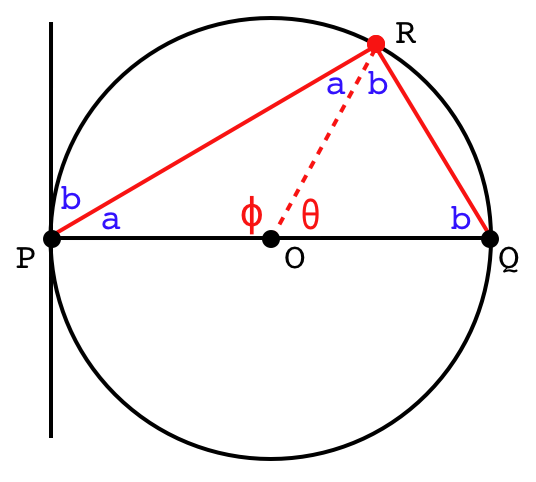
\includegraphics [scale=0.25] {arcs4.png} \end{center}
The arc between the tangent and the chord equals 2b because it is the same arc as cut off by $\angle \ PQR$ (which is $\angle \ b$).

Take a chord of the circle, draw the diameter and the tangent.
The same rule applies to both angles: one between the chord and the diameter, and the second between the chord and the tangent. The arc is twice the measure of the angle.

\subsection*{tangents}
Thales theorem provides a way to construct the tangent to a circle passing through any exterior point $P$.
\begin{center} 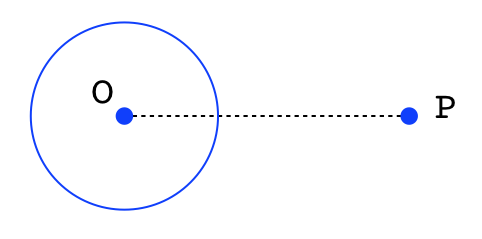
\includegraphics [scale=0.5] {tangent1.png} \end{center}
Use OP as the diameter of a circle.  Draw the line segment $OP$ and divide it in half by erecting the perpendicular bisector.  Use that distance as the radius of a new circle.  The point $R$ is the intersection of the two circles.
\begin{center} 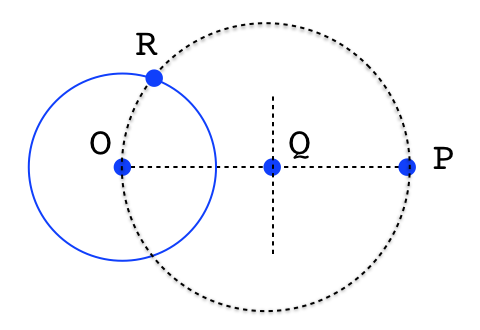
\includegraphics [scale=0.5] {tangent2.png} \end{center}

By Thales theorem, $\angle ORQ$ is a right angle, and since $OR$ is a radius of the original circle, $RQ$ is the tangent at the point $R$.

To construct a tangent on a circle at a given point $P$
\begin{center} 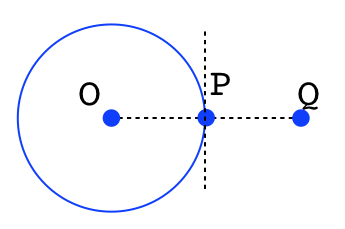
\includegraphics [scale=0.5] {tangent3.png} \end{center}
Extend $OP$ to $Q$ such that $OP$ is equal to $PQ$.  Construct the perpendicular bisector at $P$.  That is the tangent of the circle.

\end{document}